\documentclass{article}
\usepackage{geometry}
\usepackage[utf8]{inputenc}
\usepackage{hyperref}
\usepackage[table,xcdraw]{xcolor}
\usepackage{enumerate}
\usepackage{enumitem}
\usepackage{background}
\usepackage{graphicx}
\usepackage[a4paper, margin=0.9in]{geometry}
\usepackage{tikz}
\usetikzlibrary{calc}
\backgroundsetup{contents=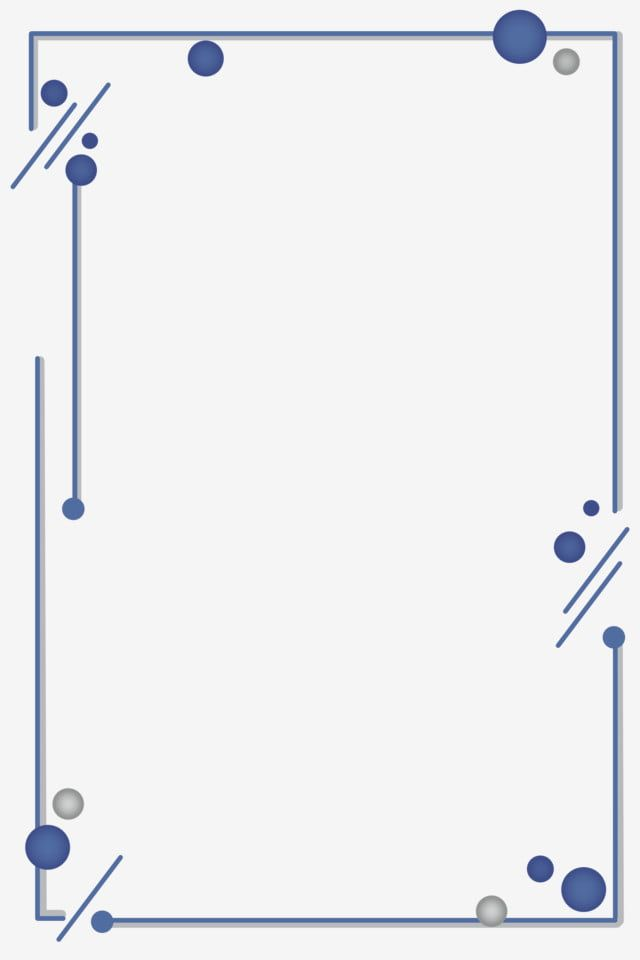
\includegraphics{background.jpeg},opacity=0.7,angle=0,scale=1}
\geometry{left=1in, right=1in, top=1in, bottom=1in}
\usepackage{titling}

\begin{document}


\begin{center}
    \huge\textbf{MAULANA ABUL KALAM AZAD UNIVERSITY OF TECHNOLOGY}\\

\end{center}
\begin{figure}[h!]
    \centering
    
\includegraphics[width=0.3\linewidth]{makaut.png}
\end{figure}
\date{\today} 
\begin{center}
    \section*{\textbf{\underline{Software Tools and Technology (Lab Notbook)}}}
    \vspace{0.4cm}
\end{center}
\begin{center}

\vspace{0.2 cm}
\renewcommand{\arraystretch}{2}
\hspace*{0.08in}
\begin{tabular}{ |c|c|c| }
\hline
\multicolumn{3}{|c|}{\Large \textbf{\textit{Group 12}}} \\
\hline
NAME & ROLL NO.& DEPARTMENT \\
\hline
Sk Shoaib Akhter [LEAD]& 30001223043& BCA \\
\hline
Urjjaswi Paul& 30059223024& Bsc in Forensic Science\\
\hline
Pranjal Paul& 30059223023& Bsc in Forensic Science\\
\hline
Rupkatha Bhowmik& 30059223009& Bsc in Forensic Science\\
\hline
Alankrita Ghosh& 30059223010& Bsc in Forensic Science\\
\hline
\end{tabular}

\end{center}
\newpage

\vspace{3cm} 
\begin{center}
    \Huge \textbf{\textcolor{black}{\underline{Table of Contents}}} 
\end{center}

\vspace{2cm} 

\begin{center}
\begin{tabular}{|>{\centering\arraybackslash}m{2cm}|m{8cm}|}
\hline
\textbf{Sl. No.} & \textbf{Questions} \\
\hline
1 & Introduction to GitHub and GitHub Desktop version installation. \\

\hline
2 & Enumerate ABC Format and Roman Number in LaTeX\\

\hline
3 & Building a C program for a calculator in the local repository, committing, and publishing it as a public repository.\\

\hline
4 & How to create matrix in LaTeX.\\

\hline
5 & Rename the button from "Submit" to "Chin Tapak Dum Dum." and create a pull request\\
\hline
\end{tabular}
\end{center}



\newpage 


\begin{center}
    \Large{\textbf{\underline{Lab -1 by Shoaib}}}
    \end{center}
    \vspace{1cm}
   \begin{center}
    \textbf{\underline{ Introduction to GitHub and GitHub installation}}
\end{center}
\begin{figure}[h!]
    \centering
    
\includegraphics[width=0.25\linewidth]{Github.png}
\end{figure}
\begin{center}
    \section*{\textbf{\underline{GitHub}}}
\end{center}


\large{GitHub is a cloud-based platform specifically designed for developers to collaborate on code and manage software projects using Git, a widely used version control system. At its core, GitHub provides a space called repositories where code is stored, allowing users to track changes over time and maintain a complete history of all updates made to the project. Through GitHub, developers can work on different features or versions of a project simultaneously by creating separate branches, which can later be merged back into the main codebase using pull requests, ensuring smooth integration of changes.}
\vspace{1 cm}
\begin{center}
    \section*{\textbf{\underline{Installation}}}
\end{center}

\large{Installing GitHub involves a few simple steps to get started with managing and collaborating on code. First, download and install Git, the version control system that GitHub uses, from the official Git website. For Windows users, run the downloaded installer and follow the prompts. On macOS, you can install Git through the terminal if it’s not already present. For Linux users, Git can be installed via the terminal with package management commands. Once Git is set up, configure it with your GitHub username and email to link your commits to your GitHub account. If you prefer a graphical interface, you can also download GitHub Desktop from its official website, which makes it easier to handle repositories, make commits, and manage branches without using the command line. After installation, sign in with your GitHub credentials or create a new account if necessary.}

\end{document}
